\documentclass[10pt]{scrartcl}
\usepackage{graphicx}
\usepackage{float}
\usepackage{amsmath}
\usepackage[utf8]{inputenc} 
\usepackage[T1]{fontenc}
\usepackage{lmodern}
\usepackage{amsfonts}   
\usepackage{amssymb}
\usepackage{mathtools}
\usepackage{epstopdf}

 
\begin{document}
\title{Praktiukumsarbeit zum Praktikum Regelungstechnik}
\author{Christian Küllmer, Jonas Kallweidt, Leon Blum}
\date{\today{}, Kassel}
\maketitle
\newpage
%Inhaltsverzeichnis
\renewcommand{\contentsname}{Inhaltsverzeichnis}
\tableofcontents
\newpage

%Mathlab Aufgabe
\section{Rechnerteil Aufgaben aus Kapitel 9.3. des Praktikumsskrips}
In diesem Anteil geht es um die in Aufgabe 9.3a. Dieser bezeichnet das Aufstellen der Gleichungen aus den gegeben Gleichungen. Die Gleichungen sind gegen als Blockschaltbild gegeben. Diese werden jetzt übersetzt in Mathlab Simulink.

%\begin{itemize}
%\item Startwerte
%Als Startwerte wurde gegeben:

%\begin{align}
%   	c &= 1 \\k &= 300  \\ T& = 0,1\\ g &= 9,81\, \frac{m}{s^2} \\l &= 1\, m\\m &= 7\, kg
%\end{align}

	
	


%\item Gegebenes Blockschaltbild:
%\begin{figure}[H]
%	\centering
%	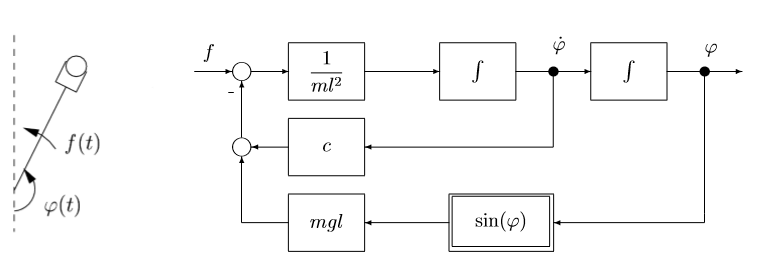
\includegraphics[width=0.6\textwidth]{Aufgabe9aMotorarm.png}
%	\caption{Motorarmmodell als Blockschaltbild}
%	\label{img:grafik-dummy}
%\end{figure}
%\begin{figure}[H]
%	\centering
%	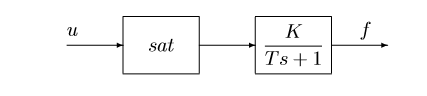
\includegraphics[width=0.6\textwidth]{Aufgabe9aStreckeMotor.png}
%	\caption{Modell des Motors als Blockschaltbild}
%	\label{img:grafik-dummy}
%\end{figure}
%\end{itemize}

\subsection{Wichtiger Hinweis:}
Für alle in diesem Bereich folgenden Auswertungen gibt folgende Farbkonvention
\begin{itemize}
\item Die rote Kurve entspricht dem Winkel $\varphi$
\item Die blaue Kurve entspricht dann der Winkelgeschwindigkeit $\dot \varphi$
\item Die grüne Kurve entspricht der Winkelbeschleunigung  $ \ddot \varphi$
\end{itemize}

%Version von Jonas und Christian vom 24.07.2019

\subsection{Aufgabe a) Gebautes Simulink Modell}
\begin{figure}[H]
	\centering
	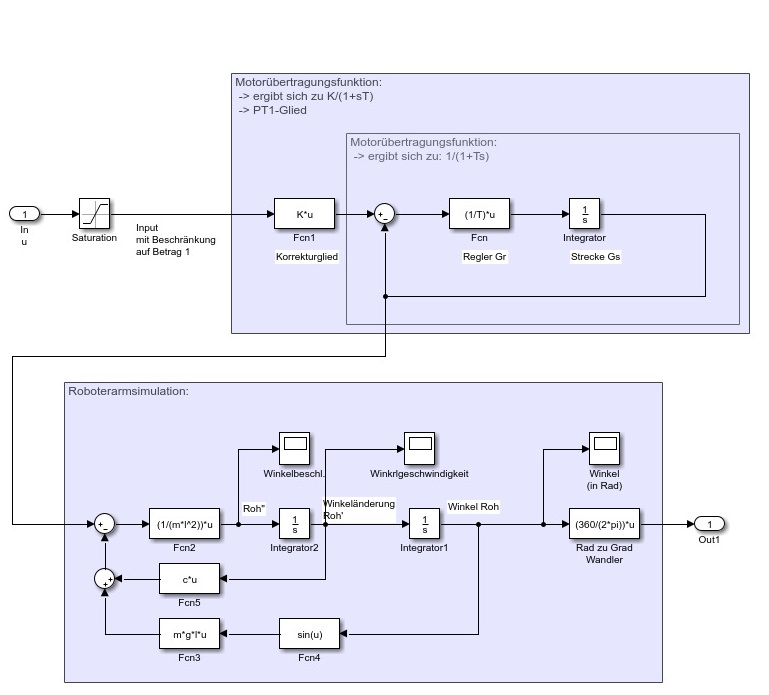
\includegraphics[width=0.7\textwidth]{Theoretischer Teil/SimulinkModell.jpeg}
	\caption{In Simulink gebautes Modell des Systems des Roboterarms}
	\label{img:grafik-dummy}
\end{figure}

%Version von Jonas und Christian vom 24.07.2019
\newpage
\subsection{Aufgabe b)}
Das System wird simuliert und die Zustandsgrößen werden über einen Zeitverlauf dargestellt. Dabei entstehen folgende Diagramme:


\begin{figure}[H]
	\centering
	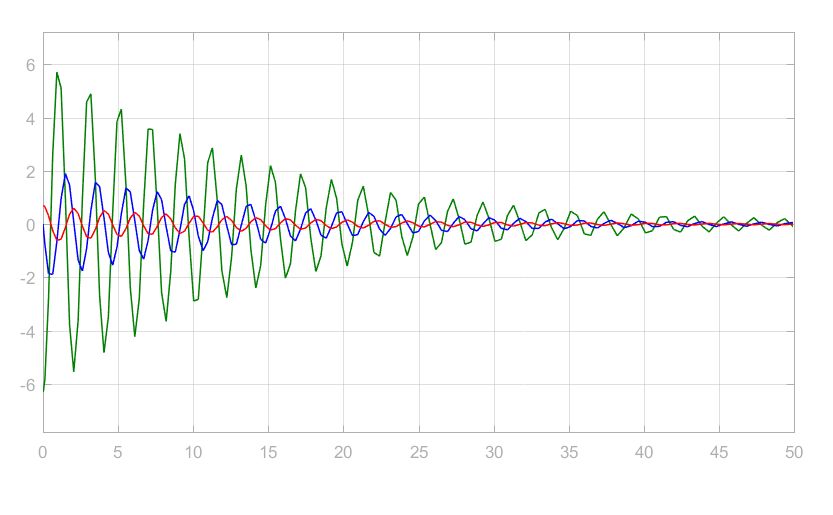
\includegraphics[width=1\textwidth]{9b}
	\caption{Darstellung des Winkels für eine anfängliche Auslenkung von 40 Grad. }
	\label{img:grafik-dummy}
\end{figure}
%Ungeregelt ist hier der Falsche Ausdruck, das was als Regelung bezeichnet wurde ist eig die Stellgröße
Aus dem Diagramm Figure 4 geht hervor, dass das System ein stabiles System darstellt,solange keine Stellgröße eingeprägt wird und dabei für gewöhlich eine Ruhelage bei 0\,$^\circ$ annehmen kann, wenn vorher keine Auslenkung vorgenommen wurde. Hier geht die Auslenkung auf keinen stationären Endwert, da die Expotentialfunktion zur Beschreibung der Dämpfung niemals null wird. In einem Realen System wird hier aber wahrscheinlich ein Stillstand nach beliebig langer Wartezeit eintreten, wenn der Roboterarm die Haftreibung nicht mehr Überwinden kann und die Bewegung im Aperiodischen Grenzfall endet.

%Version von Jonas und Christian vom 24.07.2019
\newpage
\subsection{Aufgabe c)}
Es soll eine Simulation angezeigt werden, die die Startwerte 

\begin{align}
\varphi  (0) &= 0 \\
\dot \varphi (0) &= 0 \\
u(t)  &= \binom{0\,\,\,\,\,\,\,\,\, für\,\, t<1}{0.17\,\, für\,\, t \geq 1}
\end{align}
\begin{figure}[H]
	\centering
	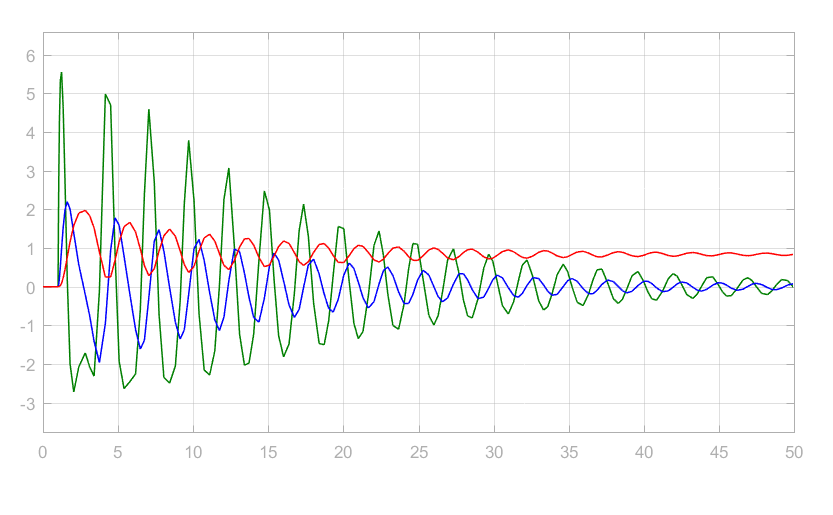
\includegraphics[width=0.8\textwidth]{9c}
	\caption{Darstellung des Winkels für eine anfängliche Auslenkung von 40 Grad. }
	\label{img:grafik-dummy}
\end{figure}
Das System befindet sich zunächst in Ruhelage
zum Zeitpunkt t=1 wird ein Drehmoment vom Motor aufgebaut,
das den Roboterarm nach Durchlaufen eines Einschwingvorgangs 
um die neue Ruhelage in eben diese auslenkt . Diese neue Ruhelage hängt von dem Eingangsdrehmoment ab. Der Einschwingvorgang hat dabei ein gleiches Verhalten, wie der Einschwingvorgang von Aufgabe 9.3.b). 


%\varphi (0) &= 0 
%f(0) &= 0 
%
%u(t) &= 0 für t<1\\
%	0.17 für t >= 1;





%Das Simulinkmodell des Roboterarms wird für die entsprechende Schaltung verändert. Alle Veränderungen werden in dieser Grafik dokumentiert.
%Danach wird das Modell linearisiert und das dann entstehende Ergebnis wird

\subsection{Aufgabe d)}
\begin{align}
\varphi  (0) &= 0 \\
\dot \varphi (0) &= 0 \\
u(t)  &= \binom{0\,\,\,\,\,\,\,\,\, für\,\, t<1}{0.18\,\, für\,\, t \geq 1}
\end{align}
\begin{figure}[H]
	\centering
	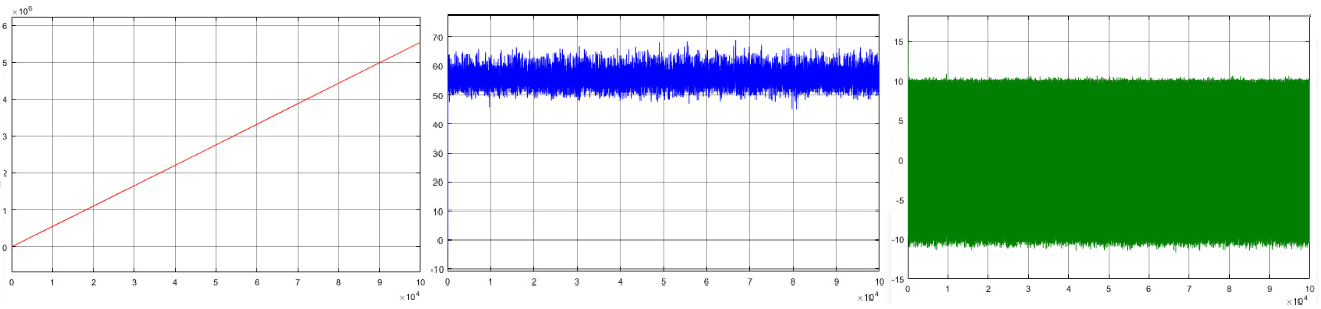
\includegraphics[width=1.2\textwidth]{Theoretischer Teil/Aufgabe9c.png}
	\caption{Darstellung des Winkels für eine anfängliche Auslenkung von 40 Grad. }
	\label{img:grafik-dummy}
\end{figure}

Anders als im Versuch 9.3c befindet sich der Roboterarm nun zum Zeitpunkt
t = 0 nicht mehr in der Ruhelage bei einem Winkel von 0\,$^\circ$, sondern in einem 
Winkel von 40\,$^\circ$. Dies hat zur Folge, dass der Arm zunächst 
in der Zeit bis t = 1*s
sowie in der darauffolgenden Sättigungszeit des PT1-Gliedes,
das den Motor beschreibt, zurückschwingen kann.
Sobald das Drehmoment des Motors aufgebaut ist legt der Roboterarm 
an Geschwindigkeit zu und überschreitet dabei sogar die kritische 180\,$^\circ$
Marke, ab der der Arm nicht mehr zurückschwingt, sondern einen Überschlag
vollführt und weiter an Geschwindigkeit gewinnt.
Da es sich bei dem betrachtetet Roboterarm um ein gedämpftes Model
handelt, geht die Gewschwindigkeit in eine Sättigung über, bis diese um
einen konstanten Wert fluktuiert. 
 %$ \alpha\beta\gamma\delta\epsilon\varepsilon\zeta\eta\theta\vartheta\iota\kappa\lambda\mu\nu\xi\pi
 %\varpi\rho\varrho\sigma\varsigma\tau\upsilon\phi\varphi\chi\psi\omega\Gamma\Delta\Theta\Lambda\Xi
 %\Pi\Sigma\Upsilon\Phi\Psi\Omega $


\subsection{Aufgabe e)}
Um zu überprüfen, ob der Motor bei einem Arm bei einem Eingangssignal von eine Ruhelage bei 40\,$^\circ$ zur Einstellung bringt. Wird dies in Mathlab mit folgendem Eingangssignal geprüft:

\begin{align}
   u_0 = \frac{m*g*l* sin( \varphi (0))}{300} = 0,1471
\end{align}
Dies entspricht einem Drehmoment von 44,1402 Nm. Dieses Drehmoment wird im Modell als Konstante Eingangsgröße Augegebenen. Der resultierende Winkel wird dann in Grad angegeben und sollte entsprechend der Erwartung einen Winkel von 40\,$^\circ$ entsprechen.
\begin{figure}[H]
	\centering
	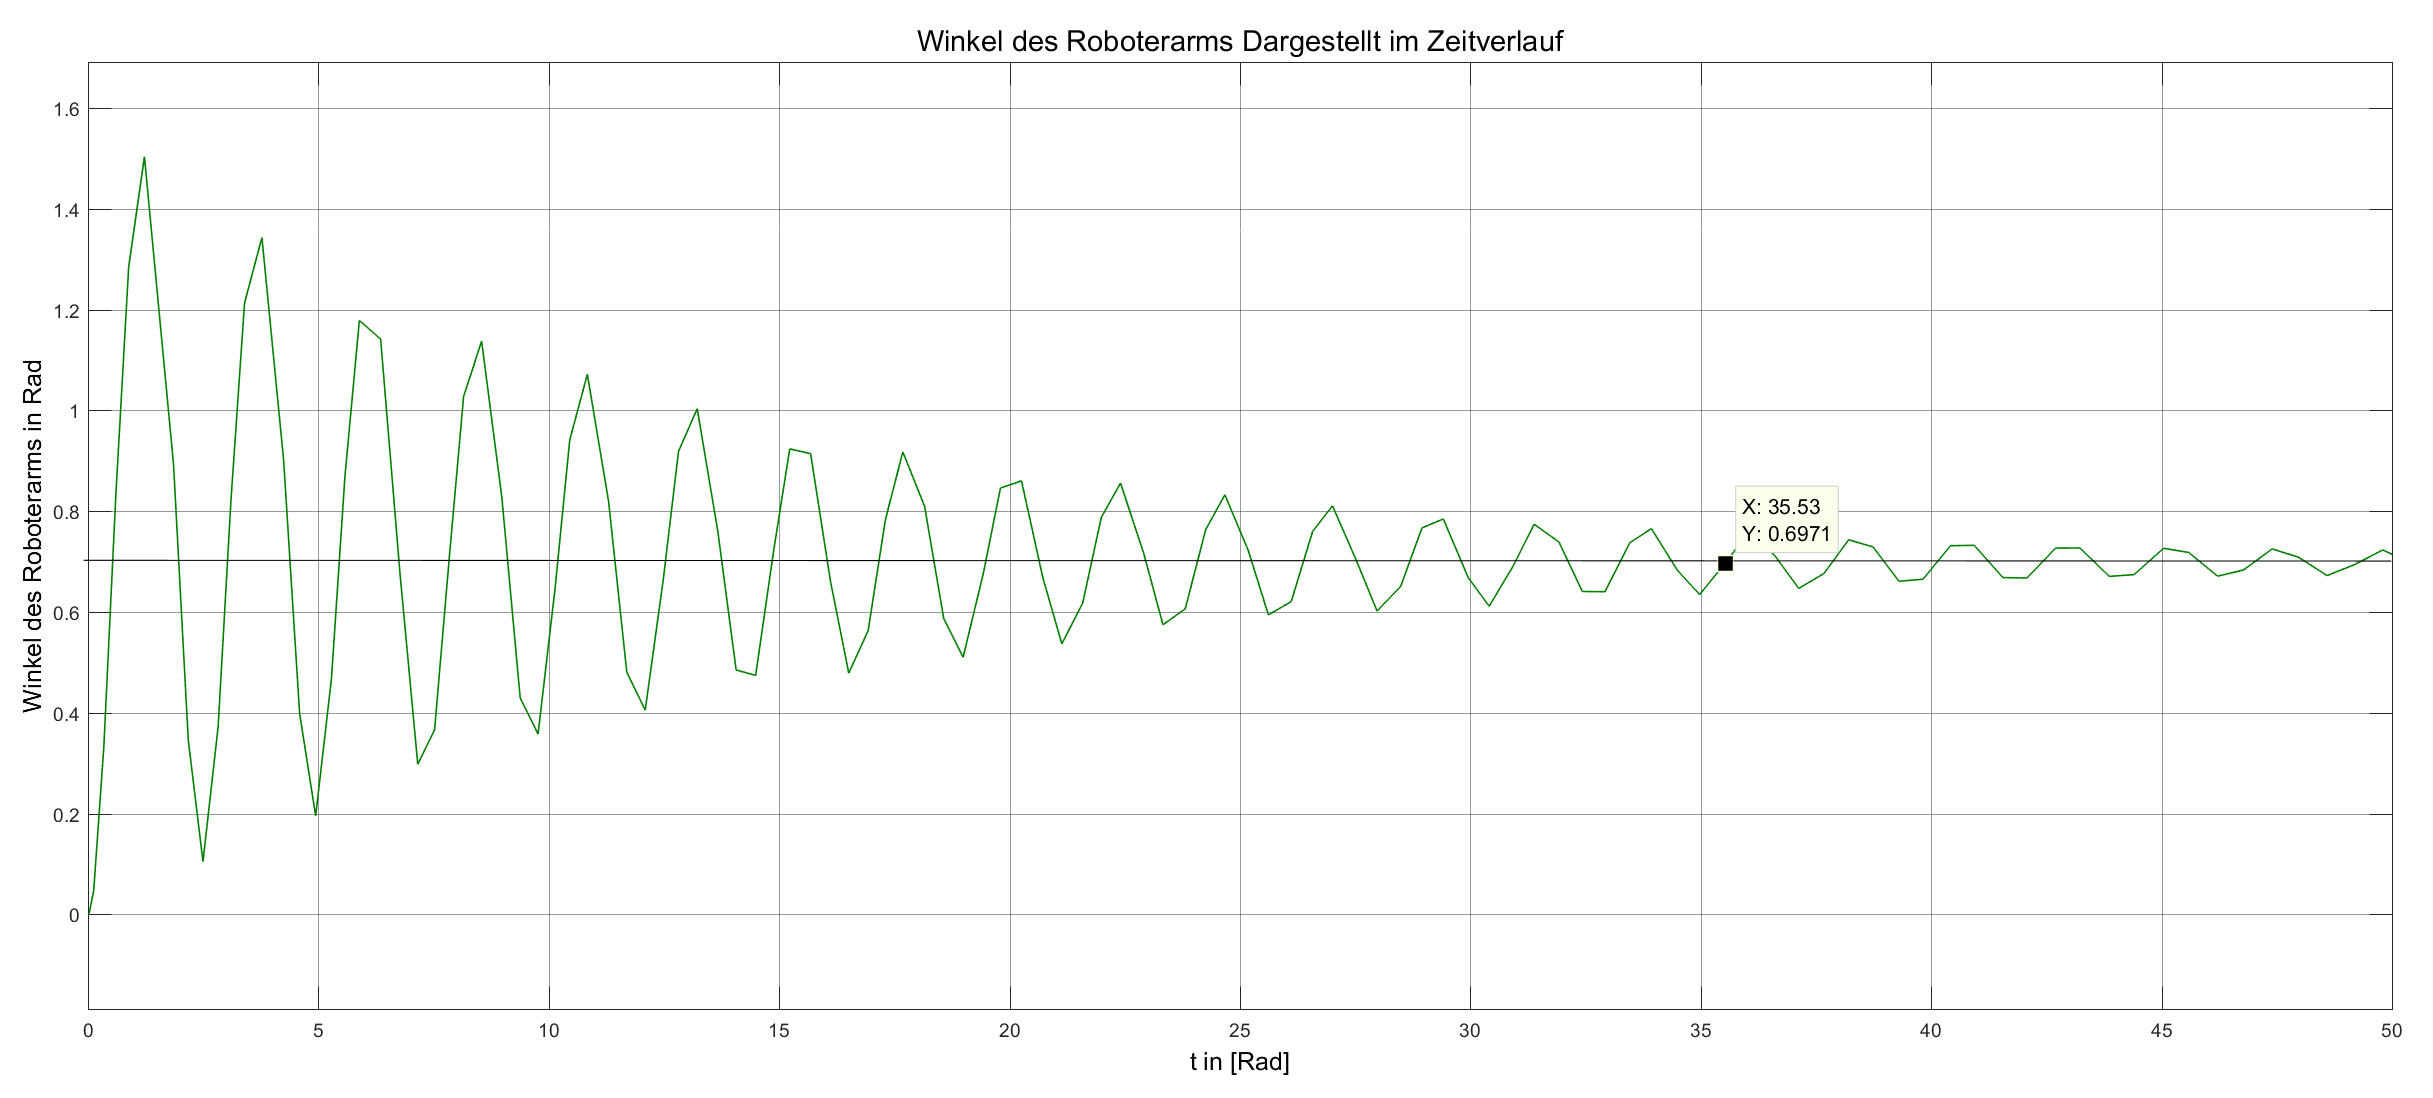
\includegraphics[width=1.2\textwidth]{Aufgabe9e}
	\caption{Darstelung des Winkelgraphen bei einem gegebenen Drehmoment}
	\label{img:grafik-dummy}
\end{figure}
An dem Diagramm ist explizit zu sehen, dass es sich bei der Auslenkung durch das Drehmoment u \textsubscript{0} einstellt. Diese Auslenkung entspricht im Mitte. einem Wert von 0,6971 Rad. Daraus ergibt sich eine neue Auslenkung von 40\,$^\circ$. Damit wird die Angabe aus dem Aufgabenscript bestätigt.


\subsection{Aufgabe f)}

Bei der Linearisirung durch Softwarenutzung von Mathlab ergibt folgendes Ergebnis im Bogenmaß:

\begin{align}
   G_s = \frac{428.6}{(s^3 + 10.14*s^2 + 8.944*s + 75.15)} 
\end{align}
Die Abweichung in der dritten Nachkommastelle des Zählers lässt sich dabei auf ein veränderten Rundungsalgorithmus im Programm verweisen. 
Die Ergebnisse stimmen also überein wodurch G\textsubscript{s} von nun an unsere Funktion der Strecke beschreibt.

\subsection{Aufgabe g)}

Um einen Regler zu finden, der die Stabilitätskriterien einhält stellen wir zunächst die orginale Wurzelortskurve dar.
\begin{figure}[H]
	\centering
	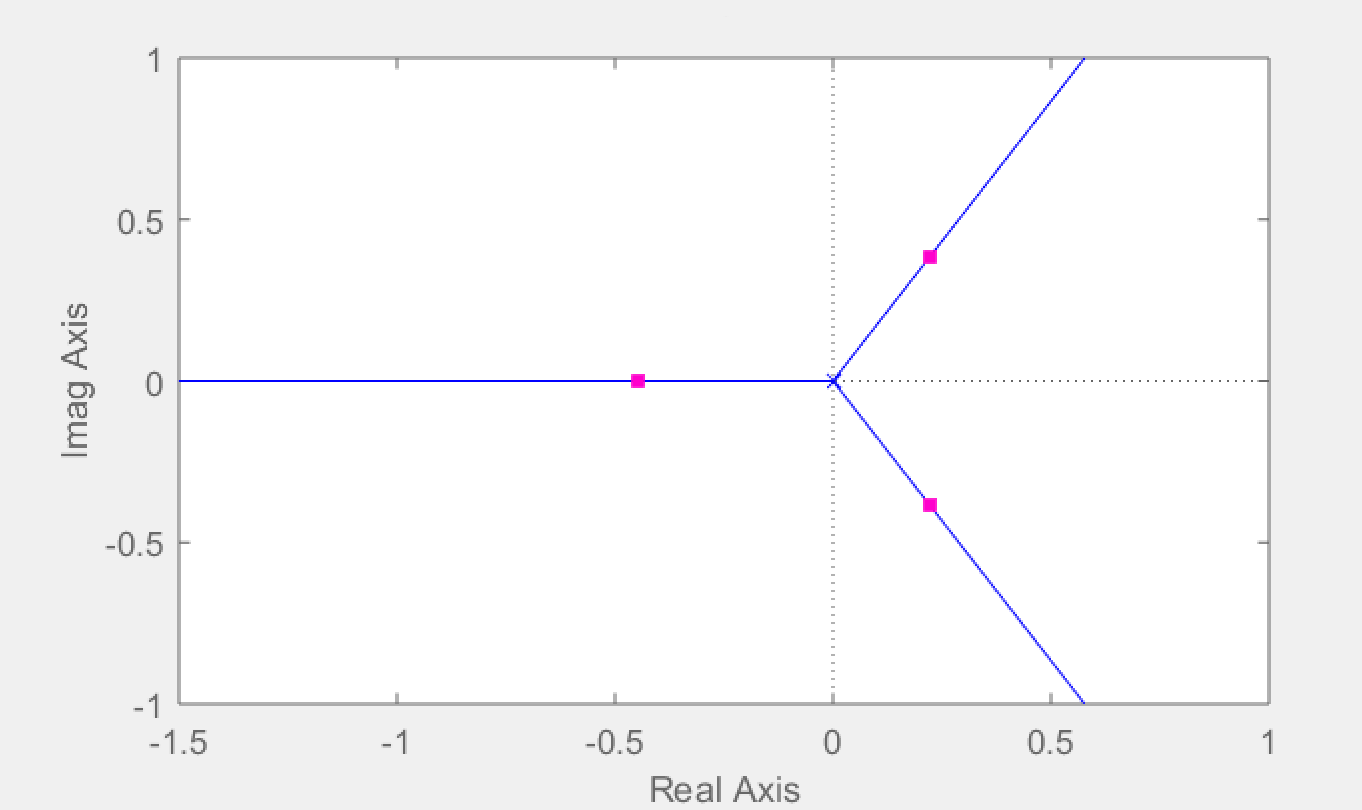
\includegraphics[width=0.8\textwidth]{WOZ9f}
	\caption{Wurzelortskurve des Systems G\textsubscript{s}}
	\label{img:grafik-dummy}
\end{figure}
In der Wurzelortskurve kann man direkt sehen, dass zwei Nullstellen in Richtung der zwei Nullstellen im positiven Bereich einen guten Reglner darstellen würden. Diese müssen dabei nicht die die Polstellen kompensieren, sondern lediglich im Imaginären Anteil des Wurzel Ortskurve liegen um dort den die Zerphilien Anteile der Wurzelortskurve anzuziehen.
Es entsteht folgende Ausgabe.
\begin{figure}[H]
	\centering
	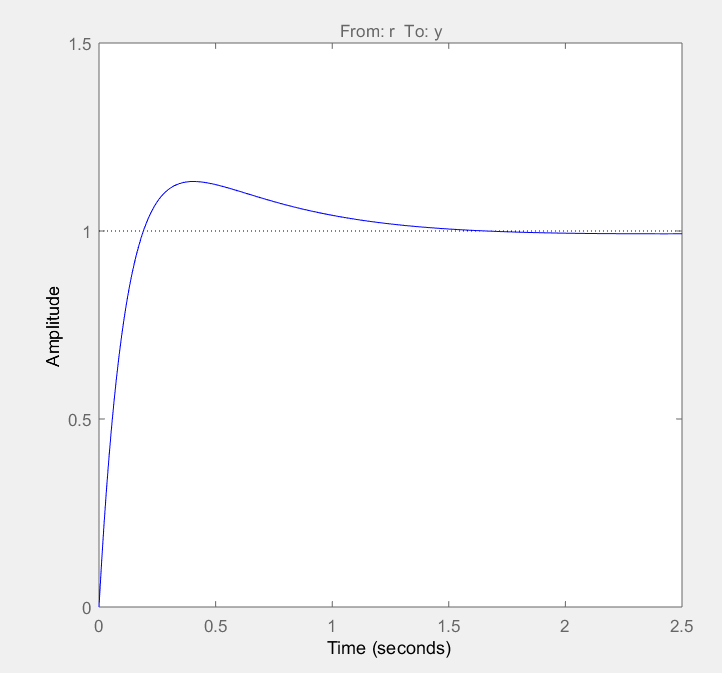
\includegraphics[width=0.6\textwidth]{WOZ9f2}
	\caption{Anzeige des Ausgangswertes}
	\label{img:grafik-dummy}
\end{figure}

Die Sich damit realisierende Ausgabe wurde von dieser Wurzelortskurve erzeugt.
\begin{figure}[H]
	\centering
	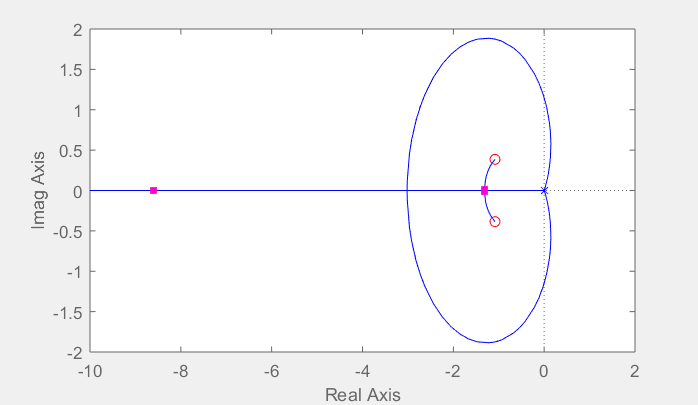
\includegraphics[width=0.8\textwidth]{WOZ9f3}
	\caption{Wurzelortskurve des Systems G\textsubscript{s} mit der Anpassung zweier Nullstellen}
	\label{img:grafik-dummy}
\end{figure}

%Präsensversuche
\section{Versuch Antrieb}

\section{Versuch Schwebekörper}

\section{Versuch Kran}
\subsection{Vorbereitungsaufgaben}
\subsection{Regelung der Wagenposition y\textsubscript{w}}
\subsection{Zusätzliche regelung des Winkels $\alpha$ }
\subsection{Digitale PD-Regelung von  y\textsubscript{w} und $\alpha$}
\subsection{Regelung mit zusätzlicher Stellgrößenbeschränkung}
\subsubsection{Einfluss der Abtastzeit}

In diesem Versuch wird der Einfluss der Abtastzeit auf das Ergebnis der Regelung genommen. Da wir die Regelfunktion des PD-Regler diskretisiert haben und danach sich das Ergebnis im k Bereich befindet, muss dieses Ergebnis dann noch in die Bildebene Z gebracht werden. 
%TODO Deltas aus dem Text entfernen!
\begin{align}
   G_R(s) = K_P + K_D s = K_P *s + K_D *·(1 + s *T_D)  \\
   y_k= K_P * k+ \frac{K_D}{T_D} *( k - 1 )  \\
   G_R(z) = K_p * z + \frac{K_D}{T_D*T} *\frac{z-1}{z}
\end{align}
Was dabei einkalkuliert wurde, ist, dass T direkt die Abtastzeit des Reglers Berücksichtigt und daraus sich der Regelkreis beeinflussen lässt.
\begin{enumerate}
\item Die Abstastzeit wird auf t = festgelegt.
\begin{figure}[H]
	\centering
	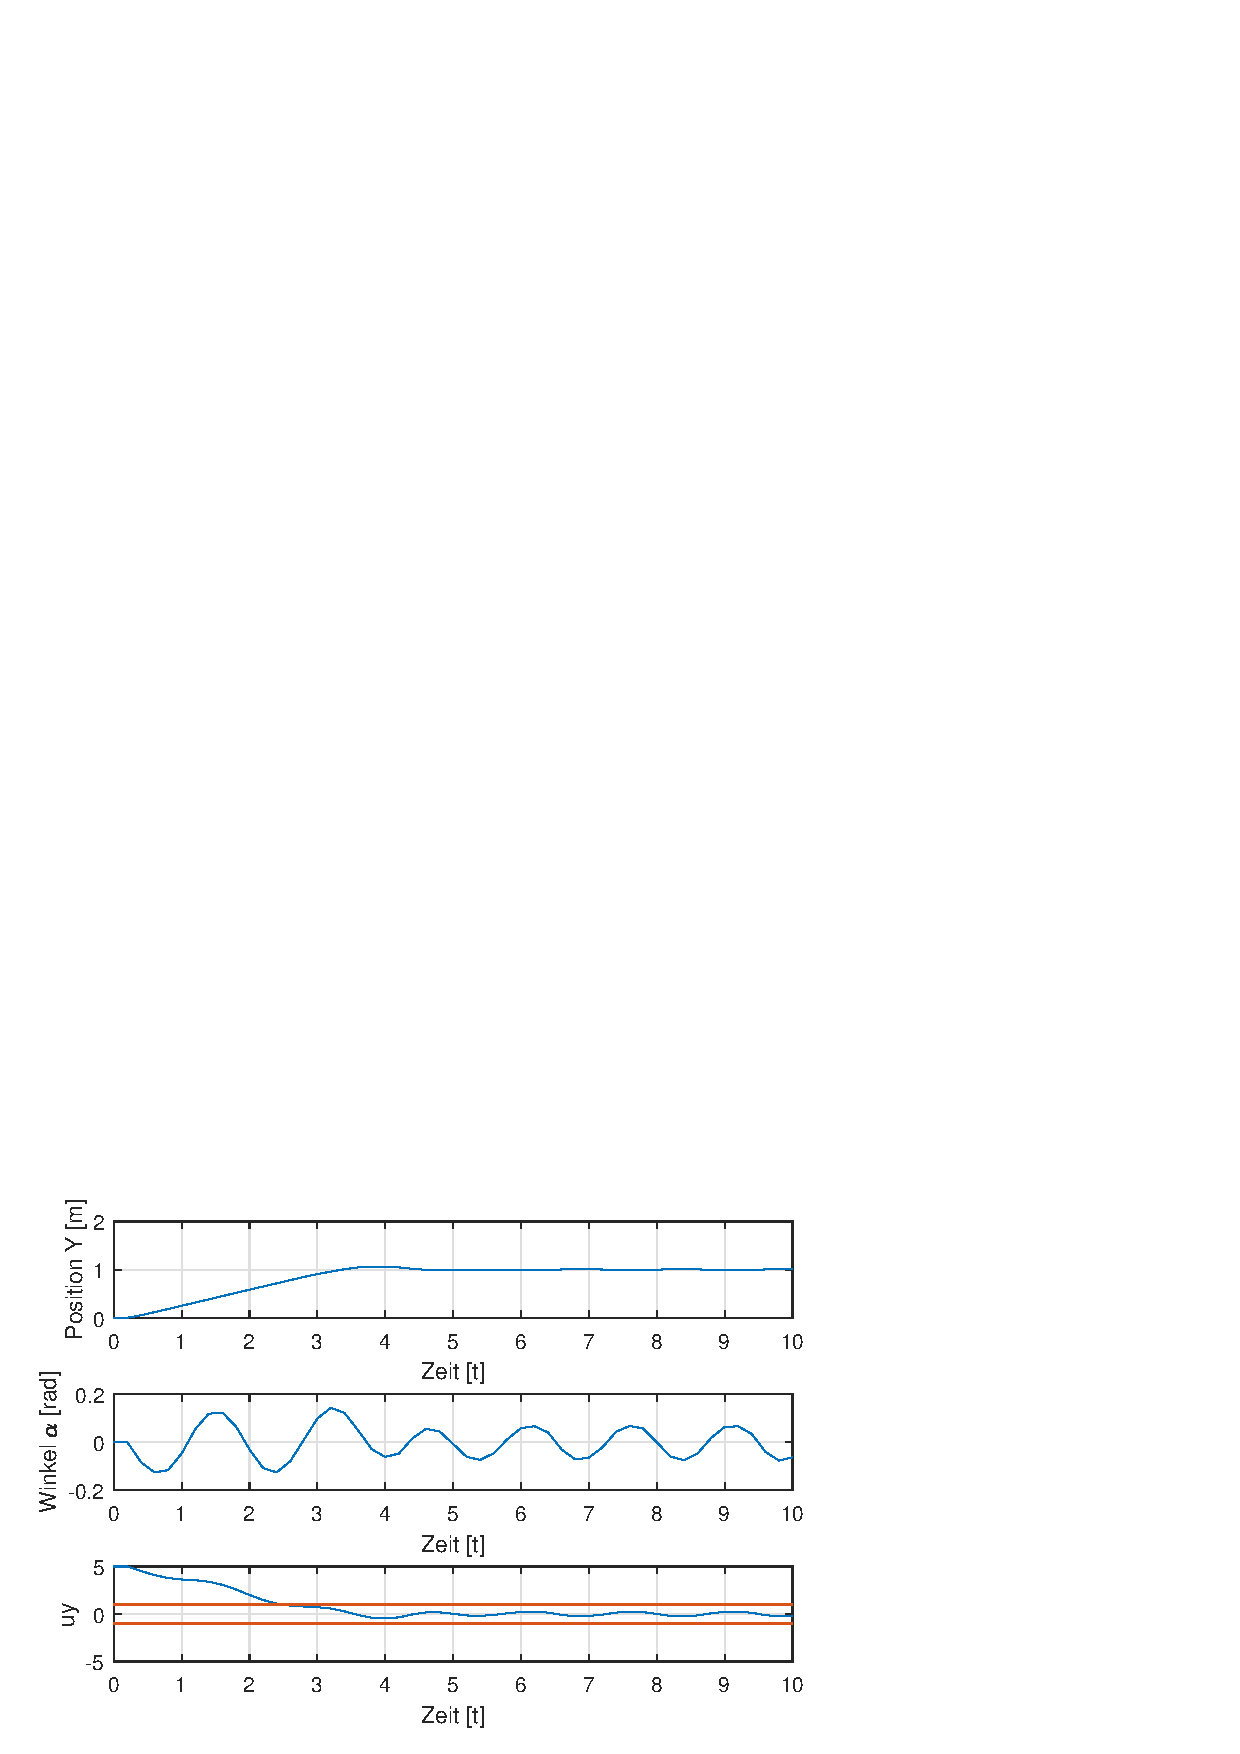
\includegraphics[width=0.8\textwidth]{Figure45a200mT}
	\caption{Verlauf des Experimentes mit einer Abtastzeit von 1ms}
	\label{img:grafik-dummy}
\end{figure}
Beobachtung:
Bei der Abtaszeit im oberen Grenzbereich schaukelt sich die eigentliche Grundbewegung auf und die Pendelbewegung wird eher verstärkt als gedämpft. Das sorgt für ein stärkere Pendelbewegung als die ungeregelte Bewegung. 
\item Die Abtastzeit wird auf t = 1 ms festgelegt.
\begin{figure}[H]
	\centering
	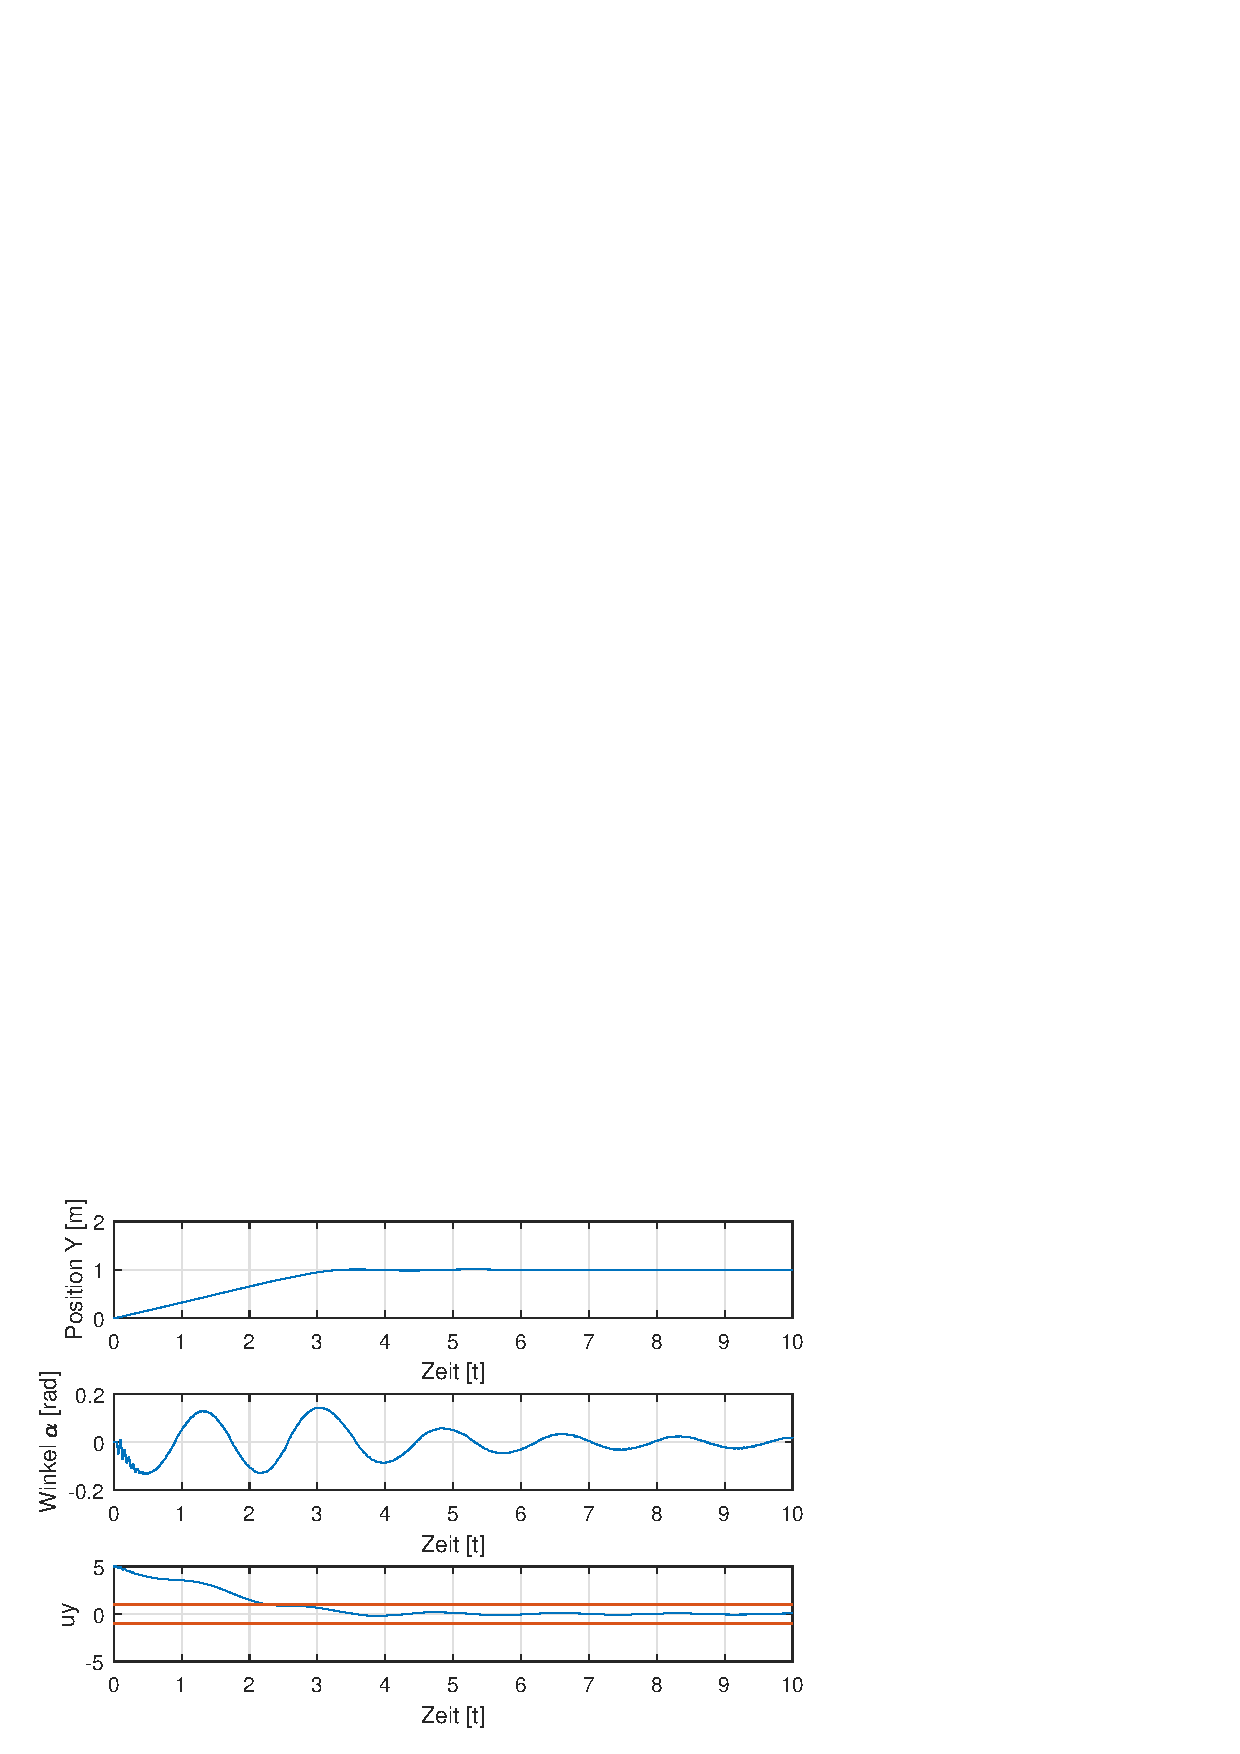
\includegraphics[width=0.8\textwidth]{45a1mT}
	\caption{Verlauf des Experimentes mit einer Abtastzeit von 1ms}
	\label{img:grafik-dummy}
\end{figure}
Beobachtung: 
Bei dieser kleineren Abtastzeit arbeitet der Regler so, dass das Schwingen des Seils stark vermieden wird. Es sorgt dafür, dass das die Auslenkung des Seils verringert wird.
\end{enumerate}
Fazit: Das Fazit, was aus diesem Versuch gezogen werden muss ist, dass die diskretisierung einer Messung und die diskretisierung eines Reglers in ausreichender Genauigkeit vorgenommen werden muss.
\subsection{Regelung der x- und y- Achse}

%Modell zum Einfügen eines Bildes
%\begin{figure}[H]
%	\centering
%	\includegraphics[width=0.8\textwidth]{}
%	\caption{Teamlogo: Team A}
%	\label{img:grafik-dummy}
%\end{figure}


\end{document}